% This is the Reed College LaTeX thesis template. Most of the work 
% for the document class was done by Sam Noble (SN), as well as this
% template. Later comments etc. by Ben Salzberg (BTS). Additional
% restructuring and APA support by Jess Youngberg (JY).
% Your comments and suggestions are more than welcome; please email
% them to cus@reed.edu
%
% See http://web.reed.edu/cis/help/latex.html for help. There are a 
% great bunch of help pages there, with notes on
% getting started, bibtex, etc. Go there and read it if you're not
% already familiar with LaTeX.
%
% Any line that starts with a percent symbol is a comment. 
% They won't show up in the document, and are useful for notes 
% to yourself and explaining commands. 
% Commenting also removes a line from the document; 
% very handy for troubleshooting problems. -BTS

% As far as I know, this follows the requirements laid out in 
% the 2002-2003 Senior Handbook. Ask a librarian to check the 
% document before binding. -SN

%%
%% Preamble
%%
% \documentclass{<something>} must begin each LaTeX document
\providecommand{\main}{.}
\documentclass[12pt,twoside]{reedthesis}
% Packages are extensions to the basic LaTeX functions. Whatever you
% want to typeset, there is probably a package out there for it.
% Chemistry (chemtex), screenplays, you name it.
% Check out CTAN to see: http://www.ctan.org/
%%
\usepackage{graphicx,latexsym} 
\usepackage{amssymb,amsthm,amsmath}
\usepackage{longtable,booktabs,setspace} 
\usepackage{chemarr} %% Useful for one reaction arrow, useless if you're not a chem major
\usepackage[hyphens]{url}
\usepackage{rotating}
\usepackage{hyperref}

\usepackage{physics}
\usepackage{siunitx}
\usepackage[subpreambles]{standalone}
% \usepackage[strings]{underscore}
% \usepackage{natbib}
% Comment out the natbib line above and uncomment the following two lines to use the new 
% biblatex-chicago style, for Chicago A. Also make some changes at the end where the 
% bibliography is included. 
%\usepackage{biblatex-chicago}
%\bibliography{thesis}

% \usepackage{times} % other fonts are available like times, bookman, charter, palatino

\title{TITLE TBD}
\author{Kees Benkendorfer}
% The month and year that you submit your FINAL draft TO THE LIBRARY (May or December)
\date{May 2021}
\division{Mathematics and Natural Sciences}
\advisor{Andrew Larkoski}
%If you have two advisors for some reason, you can use the following
%\altadvisor{Your Other Advisor}
%%% Remember to use the correct department!
\department{Physics}
% if you're writing a thesis in an interdisciplinary major,
% uncomment the line below and change the text as appropriate.
% check the Senior Handbook if unsure.
%\thedivisionof{The Established Interdisciplinary Committee for}
% if you want the approval page to say "Approved for the Committee",
% uncomment the next line
%\approvedforthe{Committee}

\setlength{\parskip}{0pt}

%%
%% End Preamble
%%
%% The fun begins:
\begin{document}

  \maketitle
  \frontmatter % this stuff will be roman-numbered
  \pagestyle{empty} % this removes page numbers from the frontmatter

% Acknowledgements (Acceptable American spelling) are optional
% So are Acknowledgments (proper English spelling)
    \chapter*{Acknowledgements}
	I want to thank a few people.

% The preface is optional
% To remove it, comment it out or delete it.
    \chapter*{Preface}
	This is an example of a thesis setup to use the reed thesis document class.
	
	

    \chapter*{List of Abbreviations}

	\begin{table}[h]
	\centering % You could remove this to move table to the left
	\begin{tabular}{ll}
		\textbf{QCD}  	&  Quantum chromodynamics \\
		\textbf{SCET}  	&  Soft collinear effective theory\\
	\end{tabular}
	\end{table}
	

    \tableofcontents
% if you want a list of tables, optional
    \listoftables
% if you want a list of figures, also optional
    \listoffigures

% The abstract is not required if you're writing a creative thesis (but aren't they all?)
% If your abstract is longer than a page, there may be a formatting issue.
    \chapter*{Abstract}
	The preface pretty much says it all.
	
	\chapter*{Dedication}
	You can have a dedication here if you wish.

  \mainmatter % here the regular arabic numbering starts
  \pagestyle{fancyplain} % turns page numbering back on

%The \introduction command is provided as a convenience.
%if you want special chapter formatting, you'll probably want to avoid using it altogether

\chapter*{Introduction}
     \addcontentsline{toc}{chapter}{Introduction}
\chaptermark{Introduction}
\markboth{Introduction}{Introduction}
% The three lines above are to make sure that the headers are right, that the intro gets included in the table of contents, and that it doesn't get numbered 1 so that chapter one is 1.

	\documentclass[../thesis.tex]{subfiles}

\providecommand{\zcut}{\mathrm{z_{cut}}}


\setlength{\parskip}{0pt}
%%
%% End Preamble
%%
%% The fun begins:
\begin{document}
\section{The physics of elementary particles}
	Modern particle physics is, ultimately, the result of a confluence of an ancient question and an ancient technique. The question: how does nature work on the most fundamental level? The technique: to smash objects together and see what comes out. 

	Of course, thousands of years of scientific development have led us to a more nuanced and sophisticated understanding than, say, the early atomic theories of Democritus and Lucretius --- though echoes of these theories remain. We now understand\footnote{Or at least, believe to understand.} that almost all visible matter and almost all observed forces are, at root, manifestations of interactions between 17 fundamental particles (though there may yet be more). We conceive of these particles as excitations in fields which permeate space-time --- this conception is known as quantum field theory.\footnote{Space-time itself is a geometric entity --- we perceive this geometry as the force of gravity, acting on both human and cosmic scales --- described by the theory of general relativity.}

	The goal of elementary particle physics\footnote{Also known simply as particle physics or high-energy physics.} is to understand these particles and fields at the deepest level.\footnote{Some particle theorists are also trying to unite quantum field theory with general relativity. Whether they will ever succeed remains to be seen, but they do lots of pretty math.} We would like to lay a complete framework, understanding their nature and their interactions to such an extent that one could, in principle, derive from first principles an explanation for any observed physical phenomenon. The field is a long way from that goal, but much progress has been made over the past centuries. Let us begin by summarizing what we know so far.

\subsection{The Standard Model}
	\begin{figure}
	\begin{centering}
		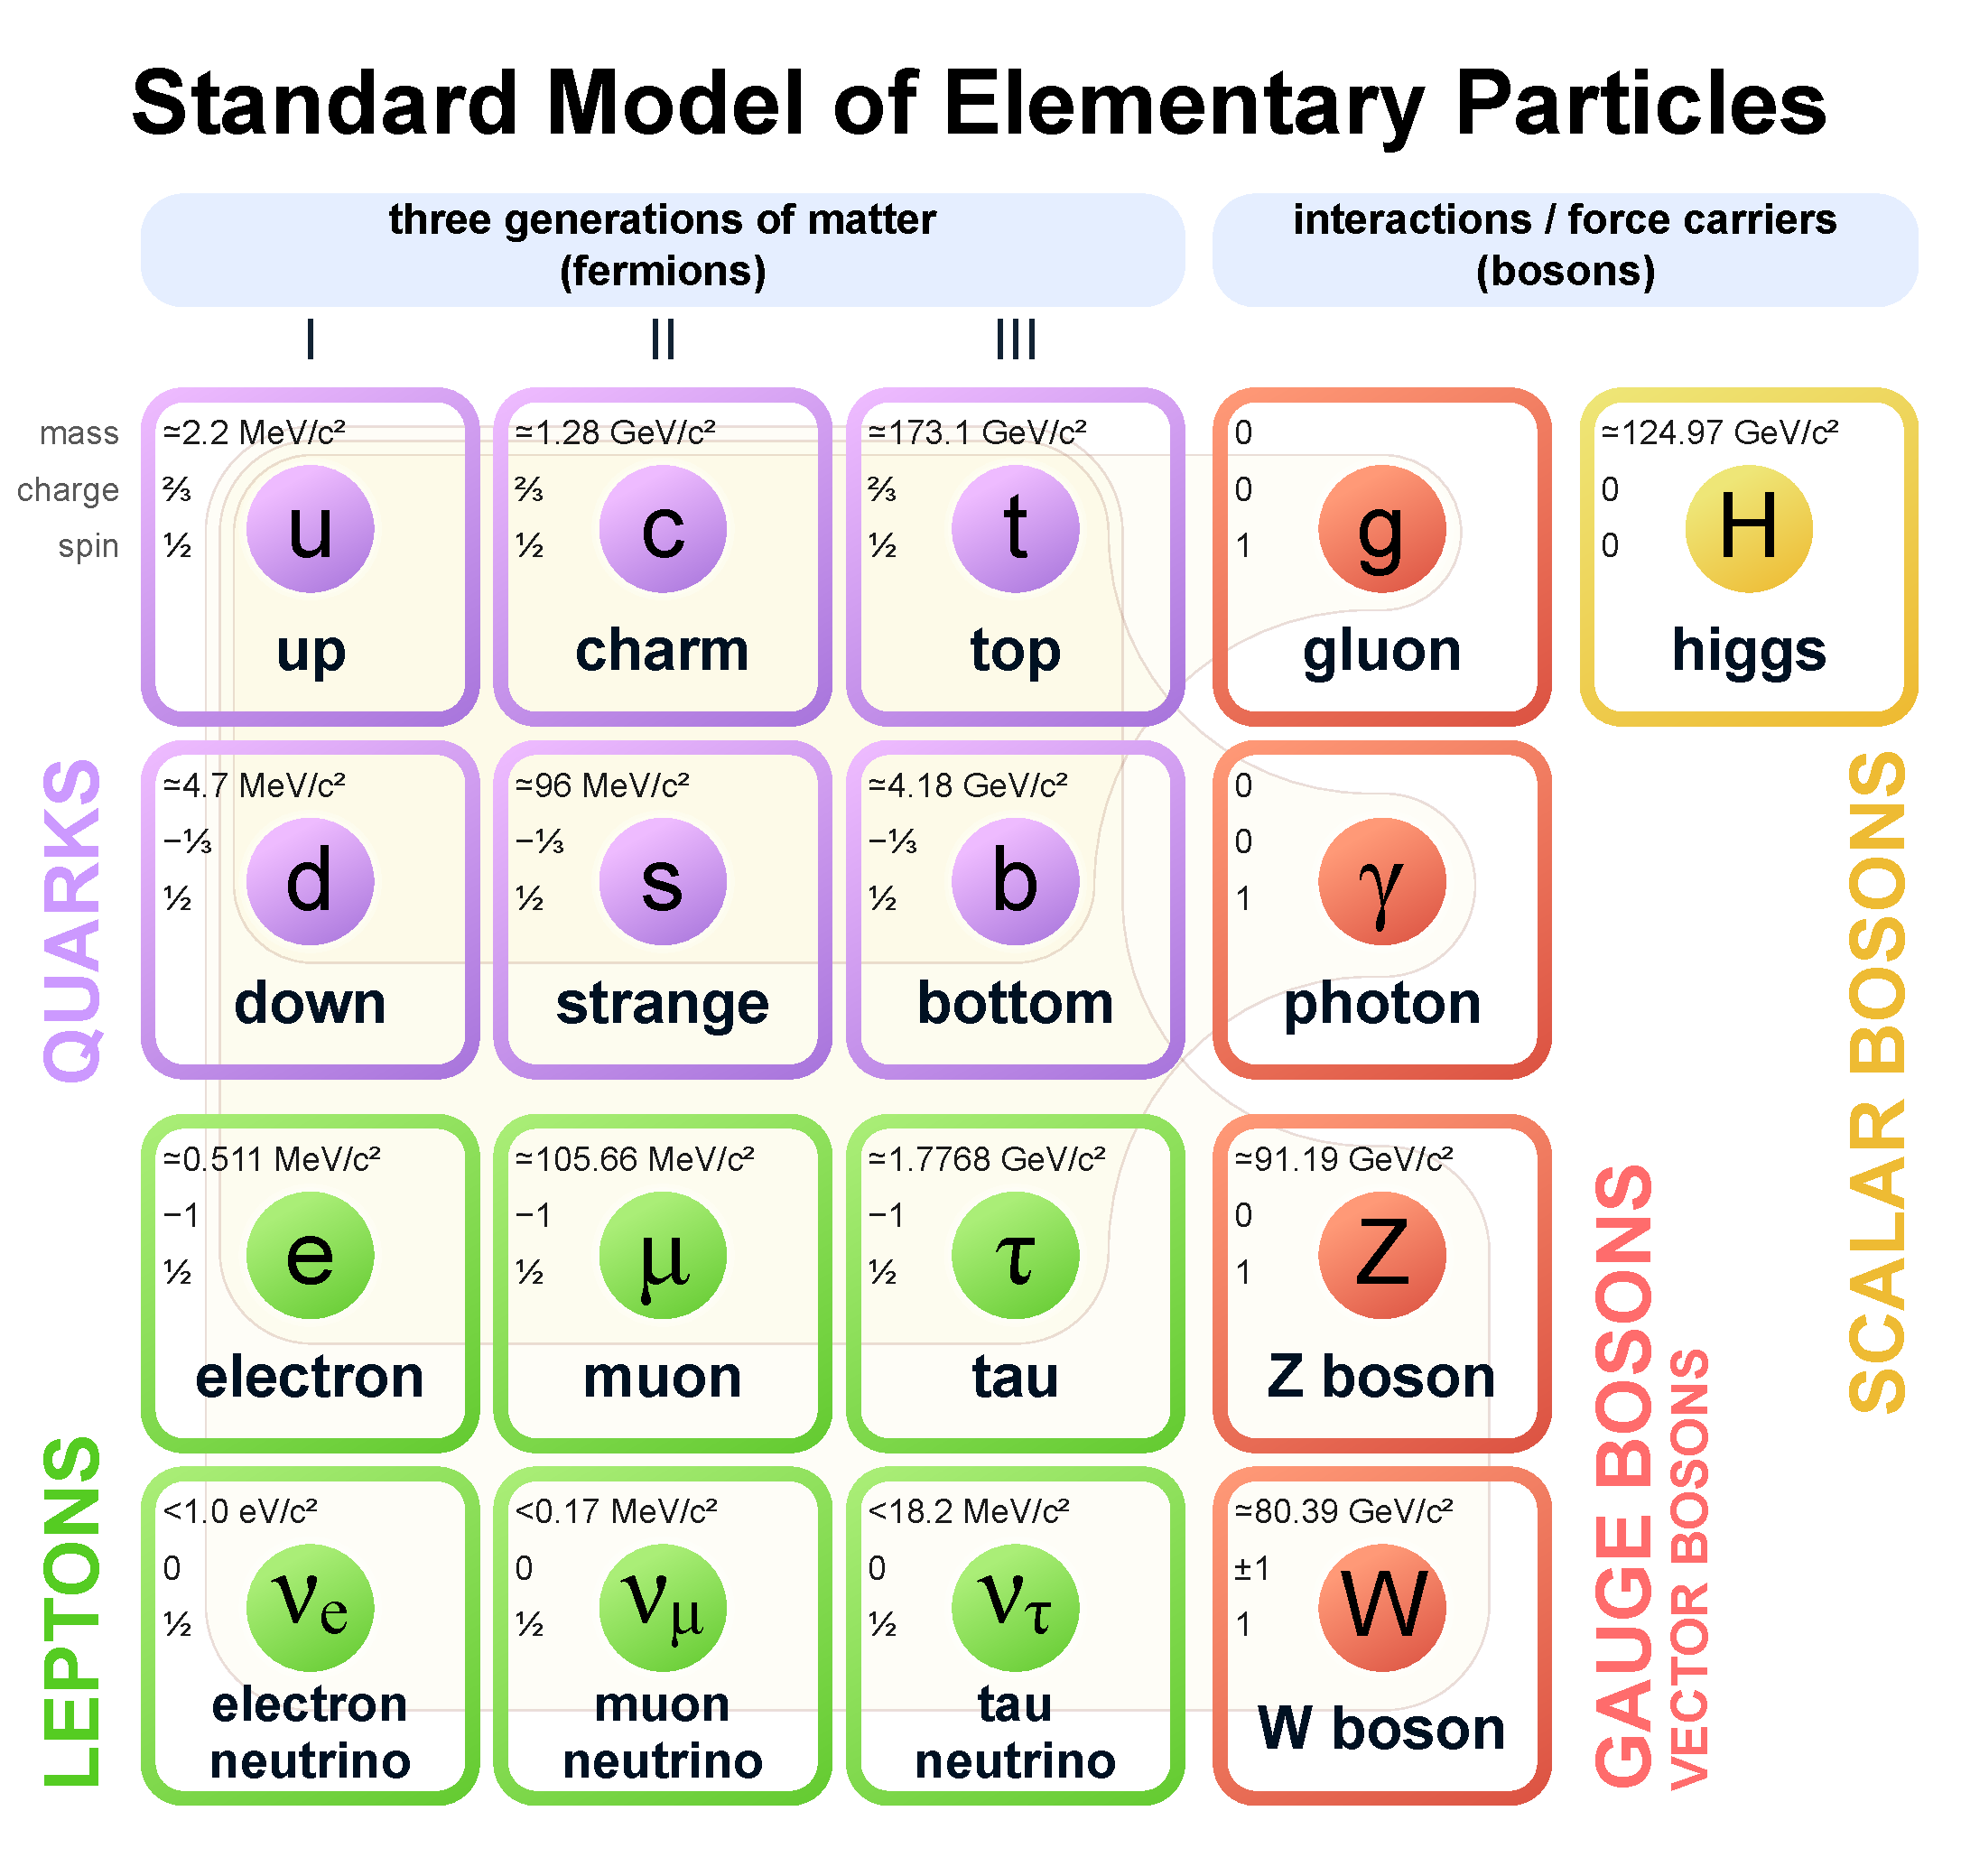
\includegraphics[width=\textwidth]{figures/Standard_Model_of_Elementary_Particles.pdf}
		\caption{\label{intro-fig:standard model}Diagram of the Standard Model of particle physics, as it currently stands. From \cite{cush_standard_2019}}
	\end{centering}
	\end{figure} 
	The 17 known particles are organized in a framework called the Standard Model of particle physics \cite{larkoski_elementary_2019-1,schwartz_quantum_2014}, displayed in schematic form in Fig.~\ref{intro-fig:standard model}.

	There are 12 particles, called \textbf{fermions}, which are the fundamental components of matter. These in turn are subdivided into \textbf{quarks} and \textbf{leptons}. Quarks, with names such as `up,' `down,' and `strange,' combine in turn to form \textbf{hadrons} --- among the hadrons are familiar composite particles like protons and neutrons. 

	The remaining 5 particles, called \textbf{bosons}, mediate interactions between particles. Four of these are responsible for three of the forces of nature: the \textbf{gluon} is responsible for the strong force; the \textbf{photon} is responsible for the electromagnetic force; and the \textbf{$W$ and $Z$ bosons} are responsible for the weak force. In terms of familiar phenomena, the strong force is what binds together the nuclei of atoms; the electromagnetic force is what makes possible most of chemistry, electronics, and modern technology; and the weak force is responsible for the decay of unstable nuclei and particles. The final boson, the \textbf{Higgs boson}, is responsible for giving mass to most of the fundamental particles, and in a technical sense is the keystone which holds the Standard Model together.

	In the Standard Model, each fermion is beholden to some subset of these bosons. The neutrinos experience the weak force and so interact via the $W$ and $Z$ bosons. The electron, muon, and tau experience the weak force as well, but they can also interact electromagnetically through exchange of photons. The quarks experience all of the fundamental forces, and can interact via any of the force-carrying bosons. It is the interaction of quarks and gluons through the strong force which will occupy most of this thesis.


\subsection{(In)completeness of the Standard Model}
	The Standard Model is a remarkable theory. It explains many observed phenomenon with unparalleled accuracy --- in fact, the Standard Model explanation of electromagnetism, called quantum electrodynamics, is the most precise physical theory ever constructed, making predictions that agree to less than 1 part per billion \cite{larkoski_elementary_2019-1}. Experiment after experiment has confirmed predictions of the Standard Model, and in this sense it is a triumph of 20th-century physics.

	In the present century, however, the strength of the theory is a significant problem in the field --- for we know that the Standard Model is incomplete. While the theory is successful at describing small-scale physics, it is not nearly as successful on a cosmic scale: it has been observed that 84.4\% of all matter in the universe is unknown to us and invisible except by gravitational signatures \cite{particle_data_group_review_2020}. We would like to understand the composition of this so-called `dark matter.' There are also more earthly hints that the Standard Model is incomplete. Among these, one of the most famous is the existence of neutrino masses. While the Standard Model describes neutrinos as massless particles, the Super-Kamiokande experiment discovered evidence in 1998 that neutrinos have a (tiny) non-zero mass \cite{super-kamiokande_collaboration_evidence_1998} --- these observations have since been verified by numerous other experiments \cite{particle_data_group_review_2020}. Finally, there are aesthetic considerations. The Standard Model, as it currently stands, has a multitude of parameters (e.g., the masses of different particles) that currently have no basis in the theory; they must be supplied externally. If possible, we would like to be able to predict these parameters eventually.\footnote{One can hardly say they understand something if, when asked why a particular detail is just so, their response is no more sophisticated than ``That's just the way it is.''}

	Thus, the Standard Model is incomplete. What can we do about that? There are two primary approaches to finding a solution:
	\begin{enumerate}
		\item \textbf{Searches for new particles:} one strategy is to design experiments that attempt to generate and detect new, previously unobserved particles. This is a well-worn technique in particle physics, responsible for many of the advances in the field over the last century. Famous examples of new-particle discoveries include the $J/\psi$ in 1974 \cite{aubert_experimental_1974,augustin_discovery_1974}, the discovery of the top quark in 1995 \cite{d0_collaboration_observation_1995,cdf_collaboration_observation_1995}, and the discovery of the Higgs boson in 2012 \cite{atlas_collaboration_observation_2012,cms_collaboration_observation_2012}. Historically, whenever new experimental frontiers have been explored, new discoveries have followed, and with them, new understanding. This is not, of course, a guarantee that such will continue in the future.\footnote{Past performance is not a guarantee of future returns.} Nevertheless, it is the underlying (if simplified) philosophy for many new particle searches at modern experiments.

		\item \textbf{Precision measurements of Standard Model parameters:} another, complementary strategy is to measure parameters of the Standard Model very precisely and then compare these measurements to theoretical predictions. These parameters could be anything from particle masses, to the strength of coupling constants, to the probability of a particular event after a particular interaction. If a discrepancy emerges, then that is a clue about where to consider modifying the Standard Model. Note, however, that to put a precise experimental measurement into a proper context, it is necessary to have at hand a precise theory. If we could measure, say, the mass of the muon\footnote{Compared to the state of the art, this would be an outrageously precise measurement. The mass of the muon is currently accepted to be \SI{105.6583745(24)}{\mega\electronvolt} \cite{particle_data_group_review_2020}, which is a precision of approximately 1 part in $10^{8}$.} to 1 part in $10^{20}$, it would do us no good if the theoretical prediction were only confident to 1 part in $10^5$. Theory and experiment must both be sufficiently advanced to take full advantage of a precise measurement.
	\end{enumerate}

	This thesis is situated firmly in the latter camp. We will be interested in precision theoretical predictions of a particular observable, called the `groomed heavy hemisphere mass,' measured in high-energy electron-positron collisions. More will be said on this topic in due time.


\subsection{Collider experiments}
	Although this thesis is theoretical in nature, it will be helpful to have some familiarity with the experiments whose outcomes we would like to predict. There is an enormous variety of experiments in particle physics, and it would be neither feasible nor helpful to discuss them all here. Instead, let us examine the two modern experiments most pertinent for our study to come. These experiments are called ATLAS (\textbf{A} large \textbf{T}oroidal \textbf{L}HC \textbf{A}pparatu\textbf{S}) and CMS (\textbf{C}ompact \textbf{M}uon \textbf{S}olenoid).\footnote{Acronyms in particle physics get very unwieldy very quickly. But look how much fun they are!} 

	Both of these are located at the Large Hadron Collider (LHC) at CERN in Geneva, Switzerland. The name of this collider is appropriate. Beams of protons are accelerated to around 99.9998\% of the speed of light using a circular ring approximately \SI{27}{\kilo\metre} in circumference.\footnote{The ring straddles the French-Swiss border.} Two beams circulate in the collider at a time, one traveling clockwise, the other counterclockwise. These beams are then maneuvered into collisions at four points around the ring, each located in the center of a massive, purpose-built experiment (in addition to ATLAS and CMS, there are two other experiments, called ALICE and LHCb). That is when the magic begins --- the collision of these protons at high energy produces, through fundamental interactions, a huge variety of particles. By observing these particles, we hope to learn something about the interactions that brought them into being.

	\begin{figure}
	\begin{center}
		\includegraphics[width=\textwidth]{figures/atlas_high_res.jpg}
		\caption{\label{intro-fig:atlas diagram}Schematic of the ATLAS experiment. For a sense of scale, note the people depicted along the bottom. Image from CERN \cite{cern_ac_layout_1998}}
	\end{center}
	\end{figure}

	ATLAS and CMS are designed as multi-purpose experiments which detect all the products of the proton-proton collisions (or at least, they try to detect them). A schematic of the ATLAS detector is displayed in Fig.~\ref{intro-fig:atlas diagram}, and a schematic of CMS is displayed in Fig.~\ref{intro-fig:cms diagram}. These detectors are built in layers surrounding the \textbf{interaction point}, with each layer serving a dedicated purpose. These layers can be summarized as follows \cite{larkoski_elementary_2019-1}:
	\begin{enumerate}
		\item In the center of each detector is the \textbf{beam pipe}. This is where collisions take place.

		\item Immediately surrounding the beam pipe is a \textbf{tracking system}. The objective of this system is to track particles as they fly away from the interaction point. From these tracks, we can glean information about the energy, charge, and type of the particles.

		\item Outside the tracking system is a \textbf{calorimetry system}. These are divided into two parts, the \textbf{electromagnetic calorimeter} and the \textbf{hadronic calorimeter}. The calorimetry system records information about the energy of particles. It works by absorbing this energy directly. The electromagnetic calorimeter is designed to most efficiently absorb particles which interact primarily through electromagnetism: electrons, photons, and the like. The hadronic calorimeter is designed to absorb hadrons like protons and neutrons.

		\item High-energy muons often escape all inner layers of the detector. Their properties are measured using \textbf{muon detectors} which line the detector's exterior.
	\end{enumerate}

	\begin{figure}
	\begin{center}
		\includegraphics[width=\textwidth]{figures/cms_160312_02.pdf}
		\caption{\label{intro-fig:cms diagram}Schematic of the CMS experiment. Note the person on the far right for scale. Image from \cite{sakuma_detector_2014}}
	\end{center}
	\end{figure}

	Using these systems, ATLAS and CMS are able to measure the results of more than a billion collision events per second, though the data is rapidly processed through a \textbf{triggering} system to reduce stored data rates to the \si{\kilo\hertz} level. \cite{atlas_outreach_atlas_2012,atlas_collaboration_performance_2017}. This data gets stored and processed at data centers distributed globally.\footnote{The scale of ATLAS and CMS is absolutely mind-boggling.} Typical searches and measurements at these experiments then look for statistical signatures of interesting physics. This could be anything from an unexpected excess of events in a particular region of phase space (for a particle search) to the probability distribution of observing particular values of particle parameters (for Standard Model measurements). 


\section{Thesis goals}
	The objectives of this thesis can be divided into two categories: scientific and pedagogical. It will be necessary to properly balance the two. Our scientific focus will be rather technical, and too much emphasis on this would cloud the narrative and make it difficult to learn from the work. The other side of this coin is that, to achieve the pedagogical goals of the thesis, we will have to complete only a partial calculation. This is not a complete loss --- what we achieve will be meaningful in its own right, and we will not have to suffer unnecessary tedium. Nevertheless, I warn the reader in advance that the story will be left incomplete.

	But enough digression --- what are the goals?

\subsection{Scientific}
	The primary scientific objective of the thesis will be to complete an all-orders calculation of the distribution of groomed heavy hemisphere mass in $e^+ e^- \to \text{jets}$ events, in the limit that the jet mass is approximately equal to the grooming cutoff. There are several moving parts here:
	\begin{enumerate}
		\item \textbf{$e^+ e^- \to \text{jets}$ events:} We are going to consider collider events in which electron and positrons annihilate to produce quarks and gluons. At high energies, because of the nature of the strong force, quarks and gluons manifest themselves in a detector as \textbf{jets}, or collimated sprays of hadronic particles. Note that these are not the type of collision events observed at the LHC, which is a proton-proton collider. Electron-positron annihilation is much easier to handle theoretically, and it turns out that we could, in principle, generalize our results to $pp$ collisions without much difficulty.

		\item \textbf{Heavy hemisphere mass:} We are interested in an observable called heavy hemisphere mass. To compute heavy hemisphere mass, one can divide a collision event into two hemispheres, measure the mass of both hemispheres, and then take the greater of the two masses.

		\item \textbf{Groomed:} When measuring an observable like jet mass, modern experiments like ATLAS and CMS must take into account significant amounts of background radiation from simultaneous events in the detector. One common technique to manage this background is to perform `jet grooming,' in which undesirable radiation is algorithmically removed from a jet. We will consider a particular grooming algorithm called the Modified Mass Drop Tagger (mMDT) \cite{dasgupta_towards_2013}, in which radiation with energy below some threshold is ignored. Such grooming can significantly alter the distribution of an observable, and it has important experimental and theoretical advantages. Understanding the effect of grooming on observables like jet mass is an active area of research.

		\item \textbf{The limit:} Jets are a phenomenon of the strong force, and the theory of the strong force is rather unwieldy. It is therefore difficult to accurately predict an entire observable distribution with only one calculation. While the distribution of groomed heavy hemisphere mass is well understood in the low-mass limit \cite{kardos_groomed_2020,kardos_two-_2020,frye_factorization_2016} and in the high-mass regime \cite{kardos_soft-drop_2018}, little study has been performed in the regime where the mass is approximately equal to the mMDT energy cutoff. Nevertheless, interesting physics occurs in this region --- whereas events throughout the distribution all rely on the production of two back-to-back quarks, this region is the one in which a third (gluon) emission just begins to be resolved above the grooming threshold. Thus, this region is our focus.

		\item \textbf{Calculation:} Just as we must perform calculations in particular limits to work with the strong force, so we must also perform calculations perturbatively, as a series expansion in the strong coupling constant $\alpha_s$. That is, if we want to compute an observable $\omega$, it is not usually feasible\footnote{At least with current theoretical techniques.} to do so with perfect precision. Instead, we can expand $\omega$ in $\alpha_s$,
		\begin{equation}
			\omega(\alpha_s) = \omega_0 + \omega_1 \alpha_s + \omega_2 \alpha_s^2 + \dots = \sum_{n = 0}^\infty \omega_n \alpha_s^n.
		\end{equation}
		Then, to compute $\omega$ to a particular desired accuracy, we can simply compute the coefficients $\omega_i$ up to a particular order in $\alpha_s$. Unfortunately, $\alpha_s$ is not a particularly small quantity, taking a value of order $0.1$.\footnote{The strong coupling constant is not actually a constant\dots\, it changes with the energy of observation. This process is called the \textbf{running} of the strong coupling \cite{larkoski_elementary_2019-1}. At the mass of the $Z$ boson, $\alpha_s(m_Z) = 0.1179(10)$ \cite{particle_data_group_review_2020}.} This means it often takes several terms to obtain a reasonable degree of accuracy.

		\item \textbf{All-orders:} That said, we are aiming to achieve an all-orders calculation of the groomed heavy hemisphere mass. This does \textit{not} mean that we will determine the distribution to infinite precision (i.e., infinite order in $\alpha_s$). Instead, it means that we will derive an expression which can be used to push to \textit{arbitrary accuracy} in $\alpha_s$, given the proper accuracy of inputs (and the proper degree of mathematical sophistication). Thus, by an `all-orders calculation,' we mean that we will develop a \textit{framework} for achieving precision results. The term `all-orders' also refers to the fact that our calculation will account for the influence of large logarithms at every order in $\alpha_s$ through the process of resummation.
	\end{enumerate}
	A more complete development of these foundational concepts will be provided in Chapter \ref{chap:technical}.


\subsection{Pedagogical}
	The primary pedagogical goal of this thesis is to understand the inner workings of a particular class of precision calculations in modern high-energy physics. The scientific objectives described above require a set of advanced theoretical tools which are interesting in their own right, but difficult to understand except through examples and context. Such tools include:
	\begin{enumerate}
		\item \textbf{Dimensional regularization:} There will be times when we must evaluate an integral which diverges when computed in the usual 4 dimensions (3 spatial dimensions and one temporal). We will get around this problem by performing such calculations in $d = 4 - 2\epsilon$ dimensions for some small $\epsilon$ \cite{schwartz_quantum_2014}. The result will still diverge if we send $\epsilon \to 0$, but operating in this way will allow us to see the divergences explicitly, and cancel them as appropriate.

		\item \textbf{Resummation:} A na\"ive series expansion of the distribution which we want to compute is plagued by corrections that take the form of logarithms of ratios of differing energy scales (e.g., the energy scale of a jet versus the energy scale of background radiation). When these scales are sufficiently different, the logarithm of their ratio becomes very large. Resummation is the process of getting a theoretical handle on these logarithmic corrections \cite{larkoski_elementary_2019-1}. The primary thrust of this thesis can be viewed, in a sense, as one large resummation calculation.

		\item \textbf{Soft and collinear effective theory (SCET):} Quantum field theory (QFT) is a remarkable description of the (subatomic) universe, but for our purposes it is too much machinery. Instead of using the full theory, we will make use of a low-energy effective theory called Soft-Collinear Effective Theory (SCET). SCET is essentially a limiting case of full QFT, useful in the regime which we will occupy ourselves. As a simpler theory, SCET has some useful properties that we will exploit.
	\end{enumerate}


\section{Technical and notational conventions}
	Before we embark, we must lay some mathematical ground rules. First, we hold Planck's constant and the speed of light to be equal to unity: $\hbar = c = 1$. It turns out that non-unity values of these quantities are, for our purposes, redundant; when converting a given quantity back to SI units, the appropriate factors of $c$ and $\hbar$ can be intuited from context. The result is that all quantities will be measured in units of energy. 

	Physics where we will be working is at the \si{\giga\electronvolt} scale and higher. Therefore, to a high degree of accuracy, we will assume all particles to be massless.

	Unless otherwise stated (and we \textit{will} eventually state otherwise), we will work in $4$ dimensions, comprising the usual three spatial dimensions and one temporal dimension. Vectors in $4$ dimensions (called four-vectors) are denoted by a Greek-letter index and take the form
	\begin{equation}
		p^\mu = (p^0, p^1, p^2, p^3).
	\end{equation}
	The $0$-th component of a four-vector is its `time' (or equivalent) component, and the others are the `spatial' (or equivalent) components. Thus, for example, a four-vector representing position would be
	\begin{equation}
		x^\mu = (t, x, y, z),
	\end{equation}
	while a four-momentum has the components
	\begin{equation}
		p^\mu = (E, p_x, p_y, p_z)
	\end{equation}
	with energy taking the place of time. It is sometimes convenient to refer to lower-dimensional pieces of a four-vector (usually two or three of the spatial components). When doing so, we will denote the sub-vector using a bold-face letter:
	\begin{equation}
		p^\mu = (E, \vb{p}), \quad \vb{p} = (p_x, p_y, p_z).
	\end{equation}

	As is standard in high-energy physics, we will neglect the effects of gravity and assume we are working in a flat space-time. When combining four-vectors, we will therefore use the `mostly minus' metric\footnote{Also known as the `West Coast' metric, among other names. The `East Coast' metric takes the opposite sign convention. Our convention here is clearly the correct one, as it results in naturally positive masses.}
	\begin{equation}
		\eta^{\mu \nu} = \begin{pmatrix}
			1 & 0 & 0 & 0 \\
			0 & -1 & 0 & 0 \\
			0 & 0 & -1 & 0 \\
			0 & 0 & 0 & -1
		\end{pmatrix}.
	\end{equation}
	We will also employ the Einstein summation notation, in which one sums over repeated indices in an expression (known as `contracting' the index). Hence, for $p^\mu = (p^0, \vb{p})$ and $k_\mu = (k_0, \vb{k})$, we have
	\begin{equation}
		k_\mu p^\mu = k_0 p^0 + k_1 p^1 + k_2 p^2 + k_3 p^3.
	\end{equation}

	With our choice of metric, there is little mechanical difference between a contravariant and a covariant four-vector; one picks up a formal minus sign in the spatial components, but that is all. We will, therefore, not distinguish between the two, and we will interchange upper and lower indices freely, bearing in mind that contracting an index negates the spatial terms of the sum. Hence, for $p^\mu = (p^0, \vb{p})$ and $k^\mu = (k^0, \vb{k})$, we will write\footnote{Sorry, Joel.}
	\begin{equation}
		k^\mu p_\mu = k_\mu p^\mu = k^\mu p^\mu = k_\mu p_\mu = k^0 p^0 - \vb{k} \cdot \vb{p}.
	\end{equation}
	The final term is the standard dot product between the three-vectors. This choice enables us to abuse notation in a convenient manner: we will often drop the Greek sub/superscript on four-vectors, and use the standard notation of linear algebra to indicate their contraction:
	\begin{equation}
		k \cdot p = k^0 p^0 - \vb{k}\cdot\vb{p}.
	\end{equation}

	Let us end with a reminder about the connection between these four-vectors and the physical world. Suppose a particle has a momentum four-vector $p^\mu$. Transforming our frame of reference to the particle's rest frame, we could write $p^\mu = (E, 0, 0, 0)$, where $E$ is the particle's energy. But then, recalling the famous relation $E = mc^2 = m$ (since we set $c = 1$), we have
	\begin{equation}
		p^2 = p \cdot p = E^2 = m^2.
	\end{equation}
	Thus, the square of a particle's four-momentum yields its squared mass. Recall now that we are assuming all particles to be massless; therefore, for any `on-shell' particle (that is, a particle that could exist on its own and not just in some quantum fluctuation), we see that $p^2 = 0$, and also that $E^2 = \vb{p} \cdot \vb{p}$.\footnote{This is not strictly an accurate proof of these properties, since massless particles move at the speed of light and one cannot boost into a light-like reference frame using Lorentz transformations. But the spirit of the argument is right, and the result is the same regardless.} This will greatly simplify our calculations later on.

	With these details out of the way, let us proceed.

% \ifstandalone
% \bibliographystyle{../bsts/myJHEP} 
% \bibliography{../jet_substructure}
% \fi
\end{document}


	

\chapter{QCD, jet grooming, and SCET}
	
	First chapter here

	\section{Quantum Chromodynamics (QCD)}

	\section{Jets}

	\section{mMDT Grooming}

	\section{Soft Collinear Effective Theory (SCET)}


\chapter{Leading-order calculation}

	\section{Setup}

	\section{Dimensional regularization}

	\section{Putting it all together}


\chapter{Factorization formula}
	
	\graphicspath{{factorization/figures/}}

	% This is the Reed College LaTeX thesis template. Most of the work 
% for the document class was done by Sam Noble (SN), as well as this
% template. Later comments etc. by Ben Salzberg (BTS). Additional
% restructuring and APA support by Jess Youngberg (JY).
% Your comments and suggestions are more than welcome; please email
% them to cus@reed.edu
%
% See http://web.reed.edu/cis/help/latex.html for help. There are a 
% great bunch of help pages there, with notes on
% getting started, bibtex, etc. Go there and read it if you're not
% already familiar with LaTeX.
%
% Any line that starts with a percent symbol is a comment. 
% They won't show up in the document, and are useful for notes 
% to yourself and explaining commands. 
% Commenting also removes a line from the document; 
% very handy for troubleshooting problems. -BTS

% As far as I know, this follows the requirements laid out in 
% the 2002-2003 Senior Handbook. Ask a librarian to check the 
% document before binding. -SN

%%
%% Preamble
%%
% \documentclass{<something>} must begin each LaTeX document
% \providecommand{\main}{..}
\documentclass[../thesis.tex]{subfiles}
% \graphicspath{{\subfix{figures/}}}
% Packages are extensions to the basic LaTeX functions. Whatever you
% want to typeset, there is probably a package out there for it.
% Chemistry (chemtex), screenplays, you name it.
% Check out CTAN to see: http://www.ctan.org/
%%
% \usepackage{graphicx,latexsym} 
% \usepackage{amssymb,amsthm,amsmath}
% \usepackage{longtable,booktabs,setspace} 
% \usepackage{chemarr} %% Useful for one reaction arrow, useless if you're not a chem major
% \usepackage[hyphens]{url}
% \usepackage{rotating}
% \usepackage{hyperref}

% \usepackage{physics}
% \usepackage{siunitx}
% \usepackage{xcolor}
% \usepackage{standalone}
% \usepackage{natbib}
% Comment out the natbib line above and uncomment the following two lines to use the new 
% biblatex-chicago style, for Chicago A. Also make some changes at the end where the 
% bibliography is included. 
%\usepackage{biblatex-chicago}
%\bibliography{thesis}

% \usepackage{times} % other fonts are available like times, bookman, charter, palatino

\providecommand{\zcut}{\mathrm{z_{cut}}}


\setlength{\parskip}{0pt}
%%
%% End Preamble
%%
%% The fun begins:
\begin{document}
	Fixed-order calculations like that of Chapter \ref{chap:leading order} are nice because of their exactness, but because of the relatively large value the strong coupling, $\alpha_s \sim 0.1$, one must go to fairly high orders to obtain precision results. At low orders, the calculations are relatively straightforward, but this quickly ceases to be the case, as the number of event topologies that one must consider increases factorially with the order of $\alpha_s$. Moreover, and more pressingly, when we compute an exclusive cross section like $\sigma(e^+ e^- \to \text{hemisphere jets})$ in the presence of mMDT grooming, external energy scales are imposed. This is problematic for QCD, which is an intrinsically scale-invariant theory, and our punishment is the appearance of logarithms of scales which might grow large in particular limits, like the limit $\rho \sim \zcut \ll 1$ which we are considering \cite{larkoski_elementary_2019-1}. All this is to say that, while fixed-order calculations are nice for developing intuition for a physical quantity, they have limitations which become quite severe in the regime in which we are interested.

	We would therefore like to develop an alternative framework for calculating the distribution of heavy hemisphere mass. The strategy we will settle on is try to develop an \textbf{all-orders calculation} of the distribution. This result will take into account contributions at every order of $\alpha_s$, and provide a mathematical structure for producing arbitrarily accurate predictions, given sufficiently precise inputs. We will get there via the process of \textbf{resummation}, which will be discussed in Sec.~\ref{all-sec:resummation} (and, indeed, will occupy most of Chapter \ref{chap:all orders}). In order to prepare for that, we must first lay some groundwork.

	The first step on the path to an all-orders calculation is to derive a factorization formula for the heavy hemisphere mass cross section, the goal being to split the cross section into terms which each depend only on a single energy scale. The basic process for doing so is laid out in technical detail in Ref.~\cite{becher_introduction_2015-1}, and an example of a similar flavor to our calculation is provided by Frye et al.\ in Ref.~\cite{frye_factorization_2016}.\footnote{Indeed, the calculation of Frye et al.\ is a more general factorization of mass-like variables in groomed jets. Setting $\alpha = 2, \beta = 0$ for their two-point energy correlation function $e_2^{(\alpha)}$ under soft drop grooming with angular exponent $\beta$ yields the mMDT-groomed jet mass $\rho$. Their factorization is valid in the limit $\rho \ll \zcut \ll 1$, whereas we are interested in the limit $\rho \sim \zcut \ll 1$.} Once the cross section has been split into functions of single energy scales, the process of resummation can begin. 

	There are two primary steps in developing a factorization formula:
	\begin{enumerate}
		\item \textbf{Power counting}: this involves determining the possible radiative modes of an event and their dominant momentum scales. The term `power counting' refers to the fact that for some momentum scale $\lambda$, different radiative modes have momenta that scale as different powers of $\lambda$.

		\item \textbf{Factorization and refactorization}: Once the different radiative modes and energy scales are identified, we can use the framework of SCET to split the cross section into a convolution of terms describing different radiative modes. These terms themselves must then be split (refactored) into convolutions of terms, each of which depends, to leading order, only on a single energy scale.
	\end{enumerate}
	In this chapter, we will follow these steps to derive a factorization formula for the heavy hemisphere mass in the $\rho \sim \zcut \ll 1$ limit.

\section{Setup}
	Recall that the hemisphere mass is defined to be
	\begin{equation}
		\rho = \frac{1}{E_J^2} \sum_{i<j} 2p_i \cdot p_j
	\end{equation}
	with $E_J$ the jet energy and the sum ranging over all pairs of particles in the jet. Expanding out the dot product, we have
	\begin{equation}\label{factor-eq:jet mass z theta}
		\rho = \frac{2}{E_J^2} \sum_{i<j} \qty(E_i E_j - \vb{p}_i \cdot \vb{p}_j) = \frac{2}{E_J^2} \sum_{i<j} E_i E_j \qty(1 - \cos\theta_{ij}) = \sum_{i<j}2z_i z_j \qty(1 - \cos\theta_{ij}).
	\end{equation}
	Here, $z_i$ and $z_j$ are the relative energy fractions of each particle and $\theta_{ij}$ is the angle between particles $i$ and $j$.

	Throughout the following discussion, with $n^\mu$ the jet direction and $\bar n^\mu$ the direction opposite the jet, we will describe momenta in light-cone coordinates
	\begin{equation}
		p^\mu = \qty(p^-, p^+, p_\perp)
	\end{equation}
	with
	\begin{align}
		p^- &= \bar n \cdot p & p^+ &= n \cdot p
	\end{align}
	and $p_\perp$ the components of momentum transverse to $n$. In these coordinates, the energy fraction with respect to total energy $E_J = Q$ is
	\begin{equation}\label{factor-eq:z light cone coordinates}
		z = \frac{p^+ + p^-}{2Q}
	\end{equation}
	and, in the collinear limit, the angle to the jet axis is $\theta \approx p_\perp / p^0$ \cite{frye_factorization_2016}.
	
	In an $e^+ e^- \to \text{jets}$ event, there are two types of emission: resolved and unresolved. The essential difference is that a resolved emission is one which manifests itself as a jet at a particular scale of observation, while an unresolved emission does not. The presence of unresolved emissions can, however, perturb observable values of a resolved emission. {\color{red}\textbf{[TODO: check that this is a reasonable description]}} 

	Suppose now that we have applied an mMDT groomer with energy fraction cutoff $\zcut$. Then every \textit{resolved} emission must satisfy
	\begin{equation}
		z_i > \zcut,
	\end{equation}
	while other emissions with $z_i < \zcut$ can only pass the groomer if they are at a sufficiently small angle to a resolved emission.

\section{Power counting}
\subsection{Resolved soft emission}
	The primary emission contributing to the jet mass in the limit $\rho \sim \zcut \ll 1$ is a gluon emission $z_i$ sensitive to both $\rho$ and $\zcut$. In the presence of a hard quark (i.e., the jet) with $z_q \sim 1$, leading contributions to the jet mass of Eq.~\ref{factor-eq:jet mass z theta} is
	\begin{equation}
		\rho \approx \sum_i 2z_i \qty(1 - \cos\theta_i)
	\end{equation}
	where $\theta_i$ is the angle of emission $i$ from the quark. Considering the case with only one such emission,\footnote{This is the one-loop contribution {\color{red}\textbf{[is this accurate?]}}.} we have
	\begin{equation}
		\rho \approx z_i \qty(1 - \cos\theta_i).
	\end{equation} 
	But since $z_i \sim \zcut$ and $\rho \sim \zcut$, this means that
	\begin{equation}
		\rho \approx \rho \qty(1 - \cos\theta_i),
	\end{equation}
	so
	\begin{equation}
		\cos\theta_i \ll 1.
	\end{equation}
	This means that
	\begin{equation}
		\theta_i \sim \frac{\pi}{2}.
	\end{equation}
	Since this emission is sensitive to $\zcut \ll 1$, we can also conclude that $z_i \ll 1$. Thus, we see that the leading contribution to the cusp region comes from a \textbf{resolved soft, wide-angle} gluon. Its momentum scales like
	\begin{equation}
		p_R \sim \zcut Q \qty(1, 1, 1).
	\end{equation}
	For future reference, let this gluon have energy fraction $z_R$ and angle $\theta_R$ from the quark axis.

\subsection{Ungroomed extra-soft unresolved radiation}
	\begin{figure}
	\begin{centering}
		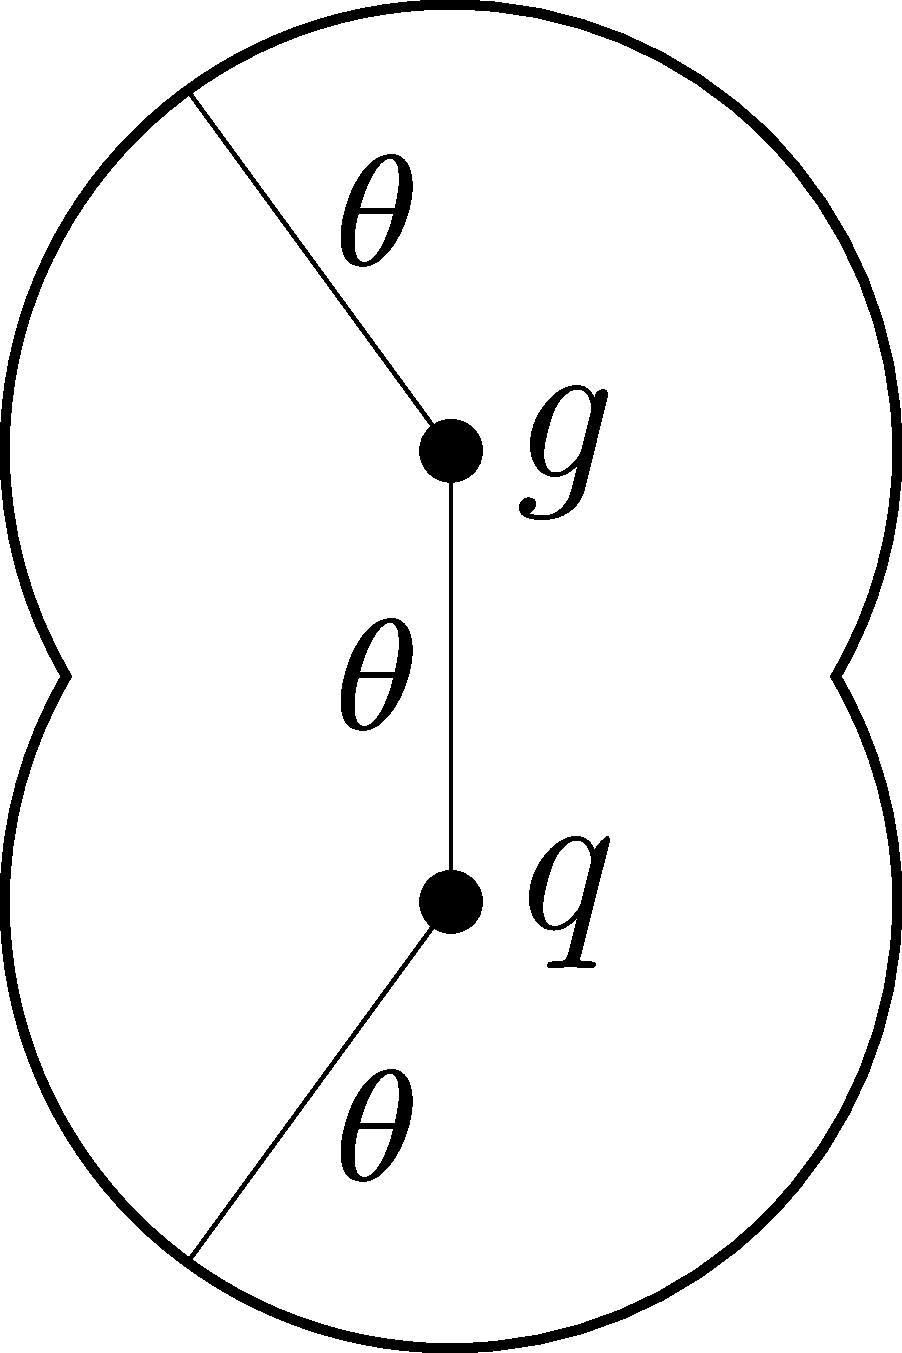
\includegraphics[width=0.2\columnwidth]{figures/head_on_schematic.pdf}
		\caption{\label{fig:head-on schematic}Head-on schematic of a quark jet $q$ and a resolved gluon $g$. If the angle between the quark and the gluon is $\theta$ and the gluon (plus all lower-scale unresolved radiation) passes the groomer, then the mMDT groomer will accept all radiation within an angle $\theta$ of both the quark and the resolved gluon.}
	\end{centering}
	\end{figure}
	Unresolved soft emissions can also contribute to the jet mass if they are sufficiently close to the resolved emission or the quark. Suppose there is another emission $i$ with energy fraction $z_i$ at angle $\theta_i$ from the jet axis and angle $\theta_{iR}$ from the resolved gluon. If $\theta_i < \theta_R$ or $\theta_iR < \theta_R$, a situation displayed in Fig.~\ref{fig:head-on schematic}, then emission $i$ will pass the groomer.

	What does this mean for the hemisphere mass? Well, first notice that since $\theta_R \sim \pi/2$, most soft radiation in the hemisphere passes this cut. The effect of these extra-soft emissions, which have $z_i \ll z_R$, is to perturb the mass of the resolved emission, so that the hemisphere mass is approximately
	\begin{equation}
		\rho \sim z_R + \sum_i z_i(1 - \cos\theta_i).
	\end{equation}
	The dominant contributions come again from the wide-angle emissions with $1 - \cos\theta_i \sim 1$; these must evidently have an energy scale set by
	\begin{equation}
		\rho - z_R \sim \sum_i z_i.
	\end{equation}
	Hence, since $z_R \sim \zcut$, the unresolved extra-soft emissions must scale as
	\begin{equation}
		p_{S_R} \sim \qty(\rho - \zcut)Q(1, 1, 1).
	\end{equation}

% \subsection{Groomed soft radiation}
% 	Radiation outside of the region displayed in Fig.~\ref{fig:head-on schematic} gets groomed away if its energy fraction is
% 	\begin{equation}
% 		z_i < \zcut.
% 	\end{equation}
% 	If $z_i > \zcut$, then we would have a second resolved emission, which we have already decided to ignore. These emissions must be at a very wide angle in order to not be within the region of mMDT acceptance. Since this \textbf{global soft} radiation is removed by the groomer, it is not sensitive to $\rho$ and contributes only to the normalization. It must scale as
% 	\begin{equation}
% 		p_{S_G} \sim \zcut Q(1, 1, 1).
% 	\end{equation}

\subsection{Collinear radiation}\label{sec:collinear radiation}
	Finally, we consider radiation collinear to a jet axis with angle $\theta_i \ll 1$. This radiation has $p^- \gg p^+$, which means from Eq.~\ref{factor-eq:z light cone coordinates} that
	\begin{equation}
		z \approx \frac{p^+}{2Q}.
	\end{equation}
	Then because the particle must satisfy
	\begin{equation}
		z_i \theta_i^2 \lesssim \rho,
	\end{equation}
	we find that \cite{frye_factorization_2016}
	\begin{equation}
		\rho \sim \frac{p^+}{Q}.
	\end{equation}

	If $z \sim 1$, we know that $z \gg \zcut$, so the momentum scales independently of $\zcut$. Hence, the scaling of these \textbf{collinear} modes is \cite{frye_factorization_2016}
	\begin{equation}
		p_c \sim Q \qty(1, \rho, \rho^{1/2}).
	\end{equation}
	In a hemisphere where the resolved emission stops the mMDT groomer, this is the only collinear radiation that contributes {\color{red}\textbf{[TODO: ask Andrew: is this correct?]}}.

	If on the other hand $z \sim \zcut \ll 1$, the result is \textbf{collinear-soft} radiation with $p^- \sim z_i Q$ and $p^+ \sim \theta_i^2 z_i Q$. From \cite{frye_factorization_2016}, these momenta scale like
	\begin{equation}
		p_{cs} \sim \zcut Q \qty(1, \frac{\rho}{\zcut}, \qty(\frac{\rho}{\zcut})^{1/2})
	\end{equation}
	and depend on the single energy scale $\sqrt{\rho\,\zcut}$. This scale matters in the hemisphere which does not contain the resolved soft gluon.


\section{Factorization}
	With the power counting in hand, we are now ready to derive a factorization formula describing the hemisphere mass distribution in the limit $\rho \sim \zcut \ll 1$. First, we should note that it is most straightforward to compute the double differential cross section in the masses of the individual hemispheres, then integrate over them to get the heavy hemisphere mass \cite{chien_resummation_2010}:
	\begin{equation}\label{factor-eq:heavy hemisphere cross section}
		\frac{d\sigma}{d\rho} = \int \frac{d^2\sigma}{d\rho_1d\rho_2}\qty[\delta(\rho - \rho_1)\Theta(\rho_1 - \rho_2) + \delta(\rho - \rho_2)\Theta(\rho_2 - \rho_1)].
	\end{equation}
	The integral simply breaks up the two cases $\rho_1 > \rho_2$ and $\rho_2 > \rho_1$ and assigns the correct value of $\rho$ in each case.

	Now, in the limit $\rho_1, \rho_2 \ll 1$, we can apply the technology of SCET to factorize the double-differential cross section into a product of hard, soft, and jet contributions \cite{frye_factorization_2016,ellis_jet_2010}. The basic form is
	\begin{equation}
		\frac{d^2\sigma}{d\rho_1 d\rho_2} = H(Q^2) \otimes S(\rho_1, \rho_2, \zcut) \otimes J_q(\rho_1) \otimes J_g(\rho_1, \zcut) \otimes J_{\bar q}(\rho_2).
	\end{equation}
	The symbol $\otimes$ represents convolution. Here, $Q^2$ is the squared center-of-mass energy of the collision. $H(Q^2)$ is hard function representing the cross section of $e^+ e^- \to q\bar{q}$ events, $S(\rho_1, \rho_2, \zcut)$ is the function representing soft contributions (which are sensitive to $\zcut$), and $J_i(\rho)$ is a function describing the production of a jet off of particle $i$ (where $i$ is a quark $q$, antiquark $\bar q$, or gluon $g$).

	As this factorization currently stands, several terms depend on multiple scales and must be refactorized. In the limit $\rho \sim \zcut \ll 1$ after mMDT grooming, the soft function consists of global soft emissions which contribute only to the normalization; a resolved soft, wide-angle emission generated by a fixed-order function; and soft radiation which passes the groomer due to the resolved emission. The first two depend only on the scale $\zcut$ and can be combined into one function. Therefore, we can write
	\begin{equation}
	\begin{aligned}
		\frac{d^2\sigma}{d\rho_1 d\rho_2} = H(Q^2) \times R(\rho_1, \rho_2, \zcut) \times S_R(\rho - \zcut) &\otimes J_{c, q}(\rho_1, \zcut)\\
			& \otimes J_{c, g}(\rho_1, \zcut) \otimes J_{c, \bar q}(\rho_2, \zcut).
	\end{aligned}
	\end{equation}
	Here, $R(\rho_1, \rho_2, \zcut)$ describes the resolved emission as well as other soft wide-angle radiation (from which the resolved emission emerged), while $S_R(\rho - \zcut)$ describes radiation which passes the groomer in the presence of the resolved emission. We have also re-written the jet functions as $J_{c, i}(\rho, \zcut)$ to make explicit their dependence on multiple scales.

	Now, as we established in Sec.~\ref{sec:collinear radiation}, radiation collinear to the jet with energy fraction of order 1 depends only on $\rho$, and radiation with energy fraction much less than 1 depends on the scale $\sqrt{\rho\,\zcut}$. However, this soft-collinear radiation only matters in the absence of a resolved gluon emission (which stops the mMDT groomer), in which case the jet function factorizes as
	\begin{equation}
		J_{c, \bar q}(\rho, \zcut) = J_{\bar q}(\rho) \otimes S_C(\sqrt{\rho\,\zcut})
	\end{equation}
	The result is that we must treat each hemisphere separately, since one contains the resolved emission and the other does not. Moreover, the gluon's jet function $J_g$ only depends on the scale of the gluon's energy, which is a function of $\rho$ and $\zcut$ {\color{red}\textbf{[TODO: check this]}}. Therefore, if we assume, without loss of generality, that $\rho_1 > \rho_2$, the cross section becomes
	\begin{equation}\label{factor-eq:factorization formula}
	\boxed{
	\begin{aligned}
		\frac{d^2\sigma}{d\rho_1 d\rho_2} = 2 H(Q^2) \times R(\rho_1, \rho_2, \zcut) &\times S_R(\rho - \zcut) \otimes J_{c, q}(\rho_1)\\
			& \otimes J_{c, g}(\rho_1, \zcut) \otimes \qty[J_{\bar q}(\rho_2) \otimes S_C(\sqrt{\rho_2\,\zcut})].
	\end{aligned}
	}
	\end{equation}
	This is our final factorization formula for the double differential cross section in each hemisphere mass. The distribution of the heavy hemisphere mass then given by Eq.~\ref{factor-eq:heavy hemisphere cross section}. We are now ready to proceed with resummation.

% \ifstandalone
% \bibliographystyle{../bsts/JHEP} 
% \bibliography{../jet_substructure}
% \fi
\end{document}



\chapter{All-orders calculation}
	Test
	

\chapter*{Conclusion}
     \addcontentsline{toc}{chapter}{Conclusion}
\chaptermark{Conclusion}
\markboth{Conclusion}{Conclusion}
\setcounter{chapter}{4}
\setcounter{section}{0}
	
	Conclusion here 


%If you feel it necessary to include an appendix, it goes here.
    % \appendix
    %   \chapter{The First Appendix}
    %   \chapter{The Second Appendix, for Fun}


%This is where endnotes are supposed to go, if you have them.
%I have no idea how endnotes work with LaTeX.

  \backmatter % backmatter makes the index and bibliography appear properly in the t.o.c...

% if you're using bibtex, the next line forces every entry in the bibtex file to be included
% in your bibliography, regardless of whether or not you've cited it in the thesis.
    % \nocite{*}

% Rename my bibliography to be called "Works Cited" and not "References" or ``Bibliography''
% \renewcommand{\bibname}{Works Cited}

%    \bibliographystyle{bsts/mla-good} % there are a variety of styles available; 
%  \bibliographystyle{plainnat}
% replace ``plainnat'' with the style of choice. You can refer to files in the bsts or APA 
% subfolder, e.g. 
 \bibliographystyle{bsts/myJHEP}  % or
 \bibliography{jet_substructure}
 % Comment the above two lines and uncomment the next line to use biblatex-chicago.
 %\printbibliography[heading=bibintoc]

% Finally, an index would go here... but it is also optional.
\end{document}
